\documentclass[runningheads]{llncs}
\usepackage[a4paper,margin=2.54cm]{geometry}
\usepackage[T1]{fontenc}
\usepackage{graphicx}
\usepackage{amsmath,amssymb}
\usepackage{booktabs}
\usepackage{float}
\usepackage{microtype}
\usepackage{xcolor}
\usepackage[hidelinks]{hyperref}
\setlength{\tabcolsep}{4pt}
\setlength{\textfloatsep}{10pt plus 2pt minus 2pt}\setlength{\floatsep}{8pt plus 2pt minus 2pt}\setlength{\intextsep}{9pt plus 2pt minus 2pt}
\setlength{\abovecaptionskip}{4pt}

\begin{document}

\title{When Does a Stride-4 Prediction Level Help a Pretrained YOLOv10 on Drone Images?}
\titlerunning{Stride-4 Level for YOLOv10 on Drone Images}
\author{Quratulain Nayeem\inst{1} \and Fahmina Taranum\inst{2} \and Mohammed Mudassir Uddin\inst{3} \and Sara Rizwan\inst{4}}
\authorrunning{Q. Nayeem et al.}
\institute{[Institution], Hyderabad, India \email{quratulainnayeem@gmail.com} \and
[Institution], Hyderabad, India \email{ftaranum@mjcollege.ac.in} \and
[Institution], Hyderabad, India \email{mohd.mudassiruddin7@gmail.com} \and
[Institution] \email{sara.rizwan014@gmail.com}}
\maketitle

\begin{abstract}
Detectors for drone imagery usually add a stride-4 prediction level to a COCO-pretrained network, and the gain is reported against baselines copied from other papers, with other schedules, input sizes and evaluation code. P2-Graft attaches a stride-4 branch to a pretrained YOLOv10, reading only the existing neck, so the original outputs are unchanged at the start, and initialises the branch from the pretrained stride-8 weights. The study covers VisDrone-DET2019 with YOLOv10n and YOLOv10s, input sizes from 640 to 1536 pixels, schedules of 35 to 150 epochs, and three seeds where compute allowed; every model is trained with one recipe on one NVIDIA RTX PRO 6000 Blackwell GPU and scored on test-dev, a split never used for model selection. At 640 pixels the branch raises test-dev AP from 14.09 to 15.77, a gain of 1.68 in every seed, and small-object AP by 2.07; validation AP reaches 20.64, above the published YOLOv8-N and FBRT-YOLO-N. The initialisation is worth 0.67 AP over a random start in a 35-epoch ablation, whereas matching weights by tensor name is not. The gain falls to 0.58 at 896 pixels and to $-$0.13 at 1280 pixels, and on YOLOv10s one seed out of three produces most of the average. The branch doubles the compute, and a baseline trained at a higher resolution is more accurate at equal GFLOPs. A stride-4 level therefore helps at small input sizes, while resolution remains the cheaper route to accuracy on VisDrone, and the initialisation of the new branch matters more than the depth of the branch.
\keywords{small object detection \and UAV imagery \and YOLOv10 \and pretrained initialisation \and VisDrone}
\end{abstract}

\section{Introduction}
Drone images are dominated by small objects. In the VisDrone-DET2019 training split~\cite{du2019visdrone}, 60.5\% of the 343,204 annotated boxes cover less than $32^2$ pixels and 26.0\% less than $16^2$. After the usual resize to a 640-pixel network input, the median box measures 10.7$\times$11.4 pixels, smaller than one cell of the stride-8 grid of the finest YOLO head.

A prediction level at stride 4 (P2) is therefore the common remedy, added on top of a detector pretrained on COCO~\cite{zhu2021tph,yang2022querydet}. The extra level needs a dedicated neck path. When the neck is re-wired to feed the level, some pretrained tensors land in layers with changed inputs, and name-based weight loading copies the tensors regardless.

Gains reported for stride-4 extensions are difficult to compare. Baselines are often copied from other papers, with other schedules, input sizes and evaluation code, and the cheapest alternative, a larger input, is rarely tried. The question addressed here is narrower: when does a stride-4 level help a pretrained YOLOv10, and what does the level cost compared with raising the resolution?

The paper makes three contributions.
(1)~\emph{P2-Graft}, a stride-4 branch reading only the pretrained neck, so the original outputs are unchanged at initialisation, with layers initialised from the stride-8 level (Sect.~\ref{sec:method}).
(2)~A controlled study of 51 training runs on one GPU with one recipe, scored from saved predictions on VisDrone test-dev, with seeds, bootstrap intervals, and baselines at the same input size and at the same GFLOPs (Sect.~\ref{sec:setup}).
(3)~A result unfavourable to the extra level: the branch adds \textbf{1.68} AP at 640 pixels, the gain shrinks as the input grows, and a plain baseline at higher resolution is better at equal compute (Sect.~\ref{sec:results}).

\section{Related Work}
\textbf{Small objects:} Feature pyramids~\cite{lin2017fpn,liu2018panet} are the standard answer to scale variation, and an extra high-resolution head is a frequent addition for drone images~\cite{zhu2021tph}. QueryDet~\cite{yang2022querydet} reduces the cost of high-resolution features with sparse queries, and slicing at inference~\cite{akyon2022sahi} trades latency for recall. Scale analyses~\cite{singh2018snip} and compound scaling~\cite{tan2019efficientnet} show input size to be a strong lever for accuracy, and input size is the lever compared with the extra level below.

\textbf{Label assignment:} Task-aligned assignment~\cite{feng2021tood} gives positives only to anchors whose centres lie inside a box. For tiny boxes the set of anchors inside the box can be empty, a gap motivating Gaussian receptive-field assignment~\cite{xu2022rfla} and Wasserstein-based similarity~\cite{wang2021nwd}.

\textbf{Growing a pretrained network:} Net2Net~\cite{chen2016net2net} widens or deepens a trained network without changing the function, and ControlNet~\cite{zhang2023controlnet} attaches new branches starting as the identity. P2-Graft carries the same idea over to the detection pyramid.

\section{Method}\label{sec:method}
\textbf{Detector:} YOLOv10~\cite{wang2024yolov10} consists of a CSP-style backbone, a PAN neck~\cite{liu2018panet} yielding the features $p_3,p_4,p_5$ at strides 8, 16 and 32, and one head per level with a one-to-many and a one-to-one branch; inference uses the NMS-free one-to-one branch. Boxes are regressed with a distribution focal loss~\cite{li2020gfl}. Under the strict centre rule of task-aligned assignment, 16.6\% of the training boxes contain no anchor centre of P3--P5 at 640 pixels, and only 3.4\% contain none once a P2 level is added. The assigner of the Ultralytics release~\cite{jocher2023ultralytics} softens the rule by enlarging boxes shorter than 16 pixels, and the default stays active for all models. Figure~\ref{fig:arch} shows the resulting pyramid, with the confident cells of each level on a real VisDrone crop.

\begin{figure}[H]
\centering
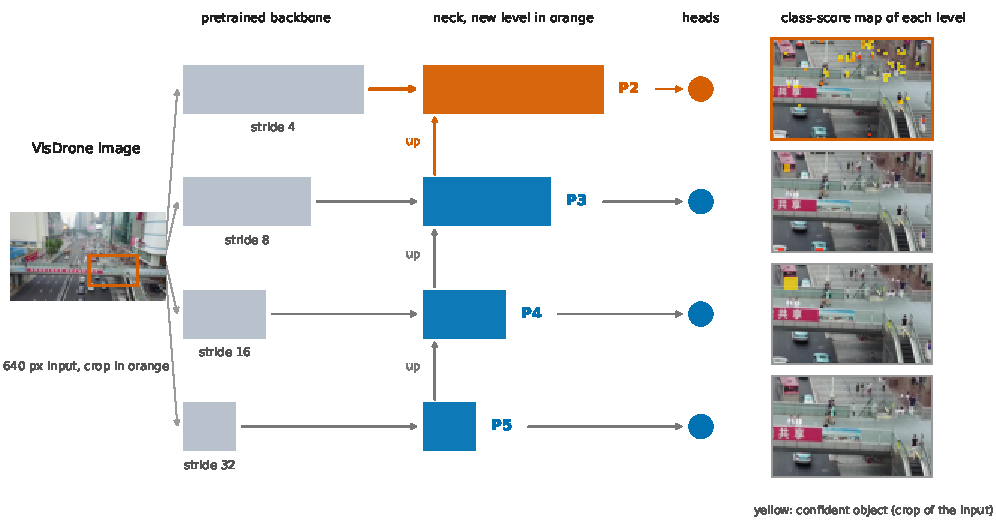
\includegraphics[width=\linewidth]{figures/fig_architecture.pdf}
\caption{Confident cells of each level on one VisDrone crop; the new stride-4 level (orange) fires on the small pedestrians.}
\label{fig:arch}
\end{figure}

\textbf{P2-Graft:} The branch extends the pyramid by one level. With $b_2$ the stride-4 backbone feature and $p_3$ the pretrained P3 neck feature, the branch computes
\begin{equation}
p_2 = G_\phi\big([\mathrm{Up}_{2\times}(p_3),\, b_2]\big), \qquad y_2 = H_\psi(p_2),
\end{equation}
where $G_\phi$ is a neck block of the type used for P3 and $H_\psi$ a detection head like the others. The new level is appended last, so layers and parameter names of the three original levels remain unchanged. No existing layer reads $p_2$ or $y_2$, hence the outputs on P3--P5 equal the outputs of the pretrained detector for any $\phi$ and $\psi$; on random inputs the maximum absolute difference over neck features and raw head outputs is exactly $0$, for YOLOv10n and YOLOv10s. All parameters are fine-tuned together afterwards.

\textbf{Warm start and depth:} A level starting at random must learn what the P3 level already knows about boxes and classes. The weights of the P3 neck block and the P3 head are therefore copied into the new block and head wherever tensor shapes agree, covering 0.22\,M parameters; the first $1{\times}1$ convolution of the block has half the input channels of the P3 counterpart and stays random. The deeper variant repeats the block twice, the second bottleneck starting as a copy of the first. Both choices were fixed by a 35-epoch search over five candidates on validation AP with one seed, and the winner, the deeper block with warm start, is called P2-Graft in the remaining sections.

\section{Experimental Setup}\label{sec:setup}
\textbf{Data:} VisDrone-DET2019~\cite{du2019visdrone} provides 6,471 training, 548 validation and 1,610 test-dev images with ten classes; ignored regions are not used as objects. Test-dev is the primary split and was never used for a decision.

\textbf{Training:} Models start from the COCO checkpoint and train with SGD (learning rate 0.01 decaying linearly to $0.01\times$, momentum 0.937, weight decay $5{\times}10^{-4}$), three warm-up epochs, mixed precision, EMA, and a nominal batch of 64 reached by gradient accumulation. Mosaic augmentation is switched off for the last epochs. Weights of the last epoch are evaluated, with no checkpoint selection. The batch is 32 up to 640 pixels; P2-Graft uses 16 from 896 pixels and 8 at 1280 pixels because the assigner memory grows with the number of anchors, while the baseline at 896 pixels keeps 32 (Sect.~\ref{sec:results} measures the effect). Some runs were interrupted and resumed from the last saved epoch.

\textbf{Evaluation:} Predictions of the one-to-one head are saved with confidence 0.001 and at most 500 boxes per image, then scored against original-resolution boxes with COCO AP~\cite{lin2014coco}. Single-seed results can mislead~\cite{bouthillier2021variance}, so gains are paired by seed. Intervals come from 200 image-level bootstrap resamples~\cite{efron1979bootstrap} of test-dev, shared by both models and applied to the seed-averaged AP.

\textbf{Hardware:} All 51 runs reported here ran on one NVIDIA RTX PRO 6000 Blackwell GPU with PyTorch 2.11 and Ultralytics 8.4.150. GFLOPs refer to the fused deploy graph.

\section{Results}\label{sec:results}
Results are reported on test-dev first, with validation AP alongside, and every gain is paired by seed. Table~\ref{tab:main} lists all comparisons.

\begin{table}[H]
\centering\small
\caption{Test-dev and validation AP (mean $\pm$ s.d. over $n$ seeds); gain is the paired test-dev difference to the baseline.}
\label{tab:main}
\begin{tabular}{llrrrrr}
\toprule
Model & Input & $n$ & GFLOPs & Test-dev AP & Val AP & Gain \\
\midrule
\multicolumn{7}{l}{\textit{YOLOv10n, 90 epochs}} \\
baseline & 640 & 3 & 6.6 & 14.09$\pm$0.09 & 17.75$\pm$0.26 & -- \\
P2-Graft & 640 & 3 & 13.7 & \textbf{15.77$\pm$0.20} & 20.64$\pm$0.09 & \textbf{+1.68} \\
\addlinespace[1pt]
baseline & 896 & 3 & 13.0 & 18.16$\pm$0.10 & 23.23$\pm$0.07 & -- \\
P2-Graft (batch 16) & 896 & 3 & 27.0 & \textbf{18.74$\pm$0.31} & 24.07$\pm$0.10 & \textbf{+0.58} \\
P2-Graft (batch 32) & 896 & 1 & 27.0 & 19.51 & 25.25 & +1.31 \\
\addlinespace[1pt]
baseline & 1280 & 1 & 27.1 & 22.45 & 28.44 & -- \\
P2-Graft & 1280 & 1 & 55.6 & 22.32 & 29.14 & \textbf{$-$0.13} \\
\addlinespace[1pt]
baseline & 1536 & 1 & 39.7 & 23.89 & 30.29 & -- \\
\midrule
\multicolumn{7}{l}{\textit{YOLOv10n, 150 epochs}} \\
baseline & 640 & 1 & 6.6 & 14.46 & 18.37 & -- \\
P2-Graft & 640 & 1 & 13.7 & \textbf{15.63} & 19.86 & \textbf{+1.17} \\
\midrule
\multicolumn{7}{l}{\textit{YOLOv10s, 90 epochs}} \\
baseline & 640 & 3 & 21.6 & 17.46$\pm$0.13 & 21.98$\pm$0.13 & -- \\
P2-Graft & 640 & 3 & 39.8 & \textbf{18.19$\pm$1.17} & 23.29$\pm$1.74 & \textbf{+0.73} \\
\bottomrule
\end{tabular}
\end{table}

\textbf{Same input size:} At 640 pixels, P2-Graft raises test-dev AP from \textbf{14.09} to \textbf{15.77}, a gain of \textbf{+1.68} with +1.53, +1.77 and +1.75 in the three seeds (Table~\ref{tab:main}, Fig.~\ref{fig:scaling}a). Small-object AP (area below $32^2$) rises by \textbf{2.07}, from 6.25 to 8.32, and validation AP by \textbf{2.89}. The gain shrinks at larger inputs: \textbf{+0.58} at 896 pixels (interval [+0.42, +0.79]) and \textbf{$-$0.13} at 1280 pixels ([$-$0.47, +0.22]). A control with batch 32 for the model (one seed) gives \textbf{+1.31} against the same-seed baseline and \textbf{19.51} AP instead of 19.09, so the smaller batch costs \textbf{0.42} AP of the 896-pixel result. Longer training does not favour the new level either: 150 epochs at 640 pixels give \textbf{+1.17}, below the 90-epoch gain.

\begin{figure}[H]
\centering
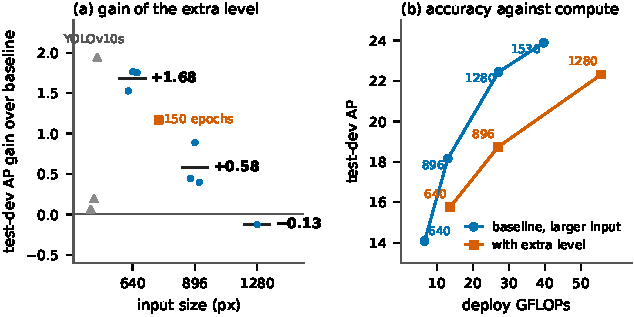
\includegraphics[width=0.8\linewidth]{figures/fig_scaling.pdf}
\caption{(a) Test-dev AP gain by input size, one dot per seed. (b) Accuracy against compute.}
\label{fig:scaling}
\end{figure}

\textbf{Resolution against the extra level:} The shrinking gain matters because P2-Graft doubles the deploy GFLOPs (13.7 against 6.6 at 640 pixels) and halves the batch-16 throughput (1,234 against 2,427 images per second at 896 pixels). Spending the same compute on resolution proves more effective. A baseline at 896 pixels costs 13.0 GFLOPs and reaches \textbf{18.16} AP, \textbf{2.39} above P2-Graft at 640 pixels. At 27 GFLOPs, the baseline at 1280 pixels reaches \textbf{22.45}, \textbf{3.71} above P2-Graft at 896 pixels (\textbf{2.94} against the batch-32 run), and the baseline keeps improving to \textbf{23.89} at 1536 pixels (Fig.~\ref{fig:scaling}b). Batch-1 latency, 3.2 to 4.0\,ms for every model on the GPU, does not separate the models.

\textbf{What matters inside the branch:} Since the extra level pays off mainly at small inputs, the internals of the branch were examined at 35 epochs (Table~\ref{tab:abl}, Fig.~\ref{fig:abl}a). With random initialisation the level adds only \textbf{+0.26}; matching weights by tensor name gives \textbf{+0.48}; the warm start gives \textbf{+0.92}, three seeds each. Depth helps only together with the warm start (\textbf{+0.26} against \textbf{+1.05}), and a third repetition adds little (+1.16, one seed). Detail injection, a strided convolution of the stride-4 feature added to the input of the P3 head for 4\% more GFLOPs, gives \textbf{+0.61} with 16 channels but only \textbf{+0.36} after 90 epochs at 640 pixels (two seeds).

\begin{table}[H]
\centering\small
\caption{Variants at 640 pixels after 35 epochs; gain is the paired test-dev difference.}
\label{tab:abl}
\begin{tabular}{lrrrrr}
\toprule
Variant & $n$ & GFLOPs & Test-dev AP & Val AP & Gain \\
\midrule
YOLOv10n baseline & 3 & 6.6 & 13.46$\pm$0.09 & 16.22$\pm$0.04 & -- \\
\midrule
P2 level, random init & 3 & 12.7 & 13.72$\pm$0.02 & 17.15$\pm$0.19 & +0.26 \\
P2 level, key-matched weights & 3 & 12.7 & 13.94$\pm$0.05 & 17.08$\pm$0.21 & +0.48 \\
P2 level, warm start & 3 & 12.7 & 14.39$\pm$0.08 & 18.05$\pm$0.02 & +0.92 \\
\midrule
2$\times$ deeper block, random init & 1 & 13.7 & 13.76 & 17.05 & +0.26 \\
\textbf{2$\times$ deeper block, warm start} & 3 & 13.7 & \textbf{14.52$\pm$0.17} & 18.48$\pm$0.05 & \textbf{+1.05} \\
3$\times$ deeper block, warm start & 1 & 14.8 & 14.66 & 18.30 & +1.16 \\
\midrule
detail injection, 16 channels & 3 & 6.9 & 14.08$\pm$0.08 & 17.16$\pm$0.21 & +0.61 \\
\midrule
P2-assisted P3, 32 channels & 1 & 8.8 & 14.49 & 17.82 & +1.00 \\
\bottomrule
\end{tabular}
\end{table}

\textbf{Second model scale:} Whether the gain carries over to a larger model was checked on YOLOv10s at 640 pixels. The mean gain is \textbf{+0.73} (interval [+0.49, +0.96]), yet the seeds give \textbf{+0.06}, \textbf{+0.19} and \textbf{+1.94} (Fig.~\ref{fig:abl}b). The standard deviation of the model across seeds is 1.17 AP against 0.13 for the baseline, so two of three seeds show no gain and the outcome is not counted as a replication.

\begin{figure}[H]
\centering
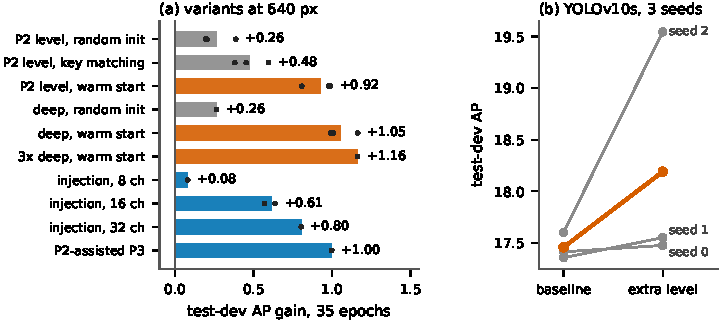
\includegraphics[width=0.8\linewidth]{figures/fig_ablation.pdf}
\caption{(a) Test-dev AP gain of each variant at 35 epochs. (b) YOLOv10s, paired seeds.}
\label{fig:abl}
\end{figure}

\textbf{Examples:} A look at individual images complements the averages. In the validation crops of Fig.~\ref{fig:qual}, chosen for the largest gain in found objects, P2-Graft finds 20 instead of 10 of 40 objects in the first crop and 21 instead of 12 of 37 in the second (score $\ge 0.3$, IoU $\ge 0.5$).

\begin{figure}[H]
\centering
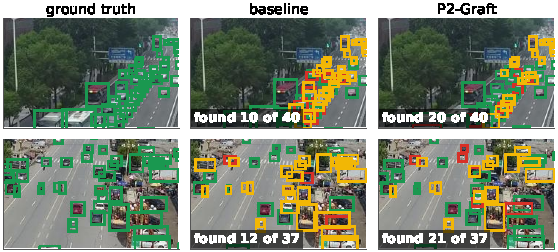
\includegraphics[width=0.74\linewidth]{figures/fig_qualitative.pdf}
\caption{Crops with the largest gain in found objects: green match, red false alarm, yellow missed.}
\label{fig:qual}
\end{figure}

\textbf{Published results:} Finally, Table~\ref{tab:lit} places the validation numbers next to results reported by other works on VisDrone. The published numbers are quoted from the respective papers, with the schedules used there (300 epochs for FBRT-YOLO), and were not re-evaluated. At 640 pixels, P2-Graft on YOLOv10n reaches \textbf{20.64} AP and \textbf{35.96} AP$_{50}$ with 2.41\,M parameters, above the reported YOLOv8-N (19.6 and 33.3, 3.2\,M) and FBRT-YOLO-N (20.2 and 34.4, 0.9\,M), after 90 epochs against 300. On YOLOv10s, the model reaches \textbf{23.29} and \textbf{39.86} against 23.8 and 39.3 reported for YOLOv10-S, a difference within the seed spread of 1.74 AP. The unmodified YOLOv10n at 1536 pixels reaches \textbf{30.29} and \textbf{49.42} with 2.27\,M parameters, above FBRT-YOLO-M (28.4 and 45.9) at an input 2.4 times larger. DroneScan-YOLO~\cite{bellec2026dronescan} also adds a stride-4 branch and trains at 1280 pixels, reporting 35.6 and 55.3, higher than every model here; the YOLOv8s baseline reported by DroneScan-YOLO scores 23.3 and 38.7 at 640 pixels.

\begin{table}[H]
\centering\small
\caption{Published validation results on VisDrone against the models of the study (bold, 90 epochs).}
\label{tab:lit}
\begin{tabular}{llrrrrl}
\toprule
Model & Input & Params (M) & GFLOPs & AP & AP$_{50}$ & Source \\
\midrule
YOLOv8-N & 640 & 3.2 & 8.7 & 19.6 & 33.3 & \cite{xiao2025fbrt} \\
FBRT-YOLO-N & 640 & 0.9 & 6.7 & 20.2 & 34.4 & \cite{xiao2025fbrt} \\
YOLOv10-S & 640 & 7.2 & 21.6 & 23.8 & 39.3 & \cite{xiao2025fbrt} \\
YOLOv8-S & 640 & 11.2 & 28.6 & 23.6 & 39.6 & \cite{xiao2025fbrt} \\
FBRT-YOLO-S & 640 & 2.9 & 22.9 & 25.9 & 42.4 & \cite{xiao2025fbrt} \\
FBRT-YOLO-M & 640 & 7.2 & 58.7 & 28.4 & 45.9 & \cite{xiao2025fbrt} \\
DroneScan-YOLO & 1280 & 10.23 & -- & 35.6 & 55.3 & \cite{bellec2026dronescan} \\
\midrule
YOLOv10n baseline & 640 & 2.27 & 6.6 & 17.75 & 31.77 & \\
\textbf{P2-Graft, YOLOv10n} & \textbf{640} & \textbf{2.41} & \textbf{13.7} & \textbf{20.64} & \textbf{35.96} & \\
YOLOv10s baseline & 640 & 7.22 & 21.6 & 21.98 & 38.16 & \\
\textbf{P2-Graft, YOLOv10s} & \textbf{640} & \textbf{7.58} & \textbf{39.8} & \textbf{23.29} & \textbf{39.86} & \\
\textbf{P2-Graft, YOLOv10n} & \textbf{1280} & \textbf{2.41} & \textbf{55.6} & \textbf{29.14} & \textbf{47.75} & \\
\textbf{YOLOv10n baseline} & \textbf{1536} & \textbf{2.27} & \textbf{39.7} & \textbf{30.29} & \textbf{49.42} & \\
\bottomrule
\end{tabular}
\end{table}

\section{Discussion}
The extra level helps where objects are small relative to the grid, i.e.\ at low input resolution. A larger input enlarges every object for the whole network, whereas the extra level adds only a finer grid on features already computed, so at equal compute the larger input wins. The gain at 640 pixels remains worth having when the input size is fixed by the camera or the latency budget, yet the gain gives no reason to prefer the extra level when the input can be raised.

Initialisation outweighs the extra layers: with a random start the branch adds \textbf{+0.26} AP, with the warm start \textbf{+0.92}, at identical cost. Consequently, any stride-4 extension of a pretrained detector should report how the new weights are initialised.

\textbf{Limitations:} Only VisDrone and two model scales were used. Results at 1280 pixels, with 150 epochs, and at 1536 pixels have one seed. The 896-pixel comparison used a smaller batch for the model, and the control measuring the effect has one seed. The model was chosen on validation among five candidates, and the validation gain exceeds the test-dev gain (\textbf{+2.89} against \textbf{+1.68} at 640 pixels), so test-dev numbers are the ones to quote. Schedules of 35 to 150 epochs are shorter than the 300-epoch recipes of the literature, and absolute values should not be compared with published tables.

\section{Conclusion}
A stride-4 level grafted onto a pretrained YOLOv10 and initialised from the stride-8 weights gains \textbf{1.68} test-dev AP at 640 pixels. The gain shrinks with input size, does not hold reliably on YOLOv10s, and costs twice the compute. For VisDrone, raising the input resolution is the better use of compute.

\textbf{Availability:} Code, per-run results and trained weights:\\ \url{https://github.com/Mudassiruddin7/YOLO}\\ \url{https://huggingface.co/datasets/mudassiruddin/yolo}

\bibliographystyle{splncs04}
\bibliography{references}
\end{document}
